\chapter{Testing}
\label{chapter:testing}
\graphicspath{ {./chapter07/Fig} }

\begin{itquote}
A stitch in time saves nine.---Anonymous
\end{itquote}


Most systems undergo testing throughout their development and before
they are delivered to the customer. Clearly, systems should be tested to
ensure that they meet the engineering requirements. In fact, one of the
desirable properties of an engineering requirement is that it be
verifiable, or in other words, testable. The philosophy of testing is
embodied in the quote above, which means that it is better to correct
errors early, rather than wait until they become much larger problems
later. As we saw in Chapter 1, the cost to correct problems increases
exponentially with the lifetime of the project. Thus, testing should be
considered throughout system development.

Testing means different things to different people. A field service
technician, assembly line worker, and designer will have their own
definitions and requirements from a test. In this chapter testing is
examined from the perspective of a systems designer intent on checking
that the system meets the engineering requirements. Along the way
fundamental testing concepts like controllability and observability are
explored. Approaches to debugging systems are provided, followed by
templates for building unit tests, integration tests, and acceptance
tests.

\section*{Learning Objectives}
\noindent\rule{\linewidth}{1pt}
By the end of this chapter, the reader should:

\begin{itemize}
\item
  Understand the concepts of black box tests, white box tests,
  observability, and controllability.
\item
  Understand the principles of debugging.
\item
  Understand when a unit test is used and how it is constructed.
\item
  Understand when an integration test is used and how it is constructed.
\item
  Understand when an acceptance test is used and how it is constructed.
\end{itemize}

\section{Testing Principles}
\label{section:testing-principles}

The design process is really a continual increase in specificity from
engineering requirements to the detailed design. We now consider the
question of how to test that the resulting system meets the design
requirements. One answer is based on a common testing model, the ``test
vee'', shown in Figure~\ref{figure:testVee}. 
This model starts with the engineering
requirements, proceeds to the implementation, and then onto testing. It
emphasizes that every level of design has a corresponding level of test.
What is not so clear from this model is that the testing process is
actually split between the two halves of the test vee. Students
typically think of testing as being exclusively confined to the right
half of the test vee -- build it then you test it. However, each test
performed in the right half of the test vee must be carefully engineered
during the development of the system in the left side of the test vee.
An acceptance test plan should be written with the Requirements
Specification, integration tests defined and written during the system
design, and so forth.

\begin{figure}
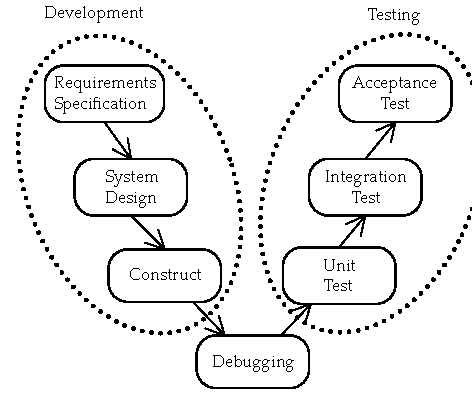
\includegraphics[width=2.9in,height=2.4in]{./image1}
\caption{The Test Vee. Design stages are on the left and
corresponding tests are on the right.}
\label{figure:testVee}
\end{figure}

In our enthusiasm to complete a project many of us all too often rely on
a ``smoke test'' -- turn on a system to see if it works. The name of
this test is a reference to what may happen to the system if the test
fails -- it burns up and smokes. Beyond being a potentially expensive
way to test a system, a smoke test is not a systematic approach to
verify that the system behaves as expected. Customer are not be
impressed with ``hey it didn't catch on fire!'' as the test result.
Clear tests need to be developed because:

\begin{itemize}
\item
  The test cases define exactly what the module must do.
\item
  Testing prevents feature creep, since the development of a module is
  complete when its test is passed.
\item
  Test cases motivate developers by providing immediate feedback.
\item
  Test cases force designers to think about extreme cases.
\item
  Test cases are a form of documentation.
\item
  Test cases force the designer to consider the design of the module
  before building it.
\end{itemize}

The test suite and its accompanying documentation contain important
information about the behavior and organization of a system and its
module. This gives tests a value beyond a role in showing that the
system and its modules do not fail the tested conditions. The individual
test cases show others engineers how to properly interface to a module,
making that module more reusable. In addition, test documents can be
used by other individuals in the organization like technical writers,
maintenance technicians, and technical trainers.

How should testing be done? Given enough time, a system could be tested
by simply enumerating every conceivable input and observing the outputs.
While in some cases this might be possible, in general it would take an
unreasonable amount of time to perform such a test. Instead, tests are
crafted in order to maximize the likelihood of finding errors.

\subsection{Types of Testing, Observability, and Controllability}
\label{subsection:types-of-testing-observability-and-controllability}

Tests fall into two general types---black box and white box tests.
\emph{\textbf{Black box tests}} are those that are performed without any
knowledge of the systems internal organization. In a black box test, the
testing is typically conducted by changing the inputs and comparing the
system outputs to their expected values. The input and output values can
be classified as typical, boundary, extreme, and invalid. These
categories are illustrated by considering a system which converts
Celsius temperatures to Fahrenheit. Typical inputs are values
experienced during normal operation, say room temperature. Boundary
values are encountered whenever the input or output changes in some
significant way. For example, 0°C and -33.3°C mark the transition
between positive to negative temperatures in Celsius and Fahrenheit
respectively. Absolute zero represents an extreme value, because things
can't get any colder. While these tests could be accomplished by
enumerate every possible input to the system and observing the output,
this would take an unreasonable amount of time. Hence, the test writer
must elect candidate inputs to represent the behavior of the system over
a range of possible inputs. An important goal of the test writer is to
minimize the number of these equivalence classes while maximizing
coverage of the input domain. Without a clear understanding of the
internal organization of the system this is a challenging goal.

\emph{\textbf{White box tests}} are conducted with knowledge of the
internal working of the system. The idea of white box testing is to
build tests which target specific internal nodes of the system to check
that they are operating as expected. The tests should be written to
check the node can handle typical, boundary, extreme and illegal
situations.

One of the many goals in designing a system is to increase its
testability. A design is \emph{\textbf{testable}} when a failure of a
component or subsystem can be quickly located. A testable design is
easier to debug, manufacture, and service in the field. One way to
increase the testability of a system is to increase controllability and
observability. \emph{\textbf{Controllability}} is the ability to set any
node of the system to a prescribed value. \textbf{\emph{Observability}}
is the ability to observe any node of a system. In black box testing,
both controllability and observability are low. In white box testing,
controllability and observability may be higher depending on the design.

Let's examine this further via the example of a simple transistor
amplifier shown in Figure~\ref{figure:transAmpDesign}. 
The purpose of this circuit, known as the
common-emitter amplifier, is to amplify the input signal,
$v_i$, to produce a linearly
proportional output signal, $v_o = A x v_i$. The
rectangular boundary in the figure represents a black box view of the
system. In this view, the system power,
$V_{cc}$, and ground would be applied to
activate the circuit. The black box testing would consist of checking
supply and ground voltages, varying the input signal, and observing the
output signal. Again, this is a low controllability and low
observability situation.

White box testing utilizes knowledge of the internal workings of the
design. When designing a transistor amplifier, there are two major
points to consider---the DC bias voltages in the circuit and its AC, or
time varying, amplification behavior. The two behaviors are related
since the AC behavior depends upon proper DC biasing of the circuit.
During detailed circuit design, the expected DC voltages for different
nodes in the circuit would be determined. Thus, a white box test would
consist of first checking the power supply and ground voltages as was
done in the black box case. The next step would be different in that the
node voltages ($V_B, V_C, V_E$) would be checked
to see if they meet the expected design values. This indicates a high
degree of observability. However, the controllability is not
significantly better than in the black box case. This is because the
internal DC node voltages in the circuit cannot arbitrarily be changed
without negatively changing the operation of the circuit.

\begin{figure}

\includegraphics{./image6}
\caption{Transistor amplifier design.}
\label{figure:transAmpDesign}
\end{figure}

\subsection{Stubs}
\label{subsection:stubs}

A \emph{\textbf{stub}} is a device that is used to simulate a
subcomponent of a system. This might be done for two reasons, either the
subcomponent has not yet been built, or the risk of damaging the
subcomponent warrants using a stand-in. Typically, stubs are used to
simulate inputs or monitor outputs of the \emph{\textbf{unit under
test}} (UUT). Both hardware and software stubs can be used when
designing a system. In software testing stub routines are developed to
either call other functions or act as those to be called by the unit
under test.

Consider a hardware example, the transistor amplifier in 
Figure~\ref{figure:transAmpDesign}.
Assume that the circuit is ultimately to be integrated into a larger
system. The input to this system is a time-varying source with certain
resistive and capacitive characteristics, while the output is connected
to another system with a known input resistance range. The stubs used
for testing in this system are shown in Figure~\ref{figure:usingStubs}. 
On the input side is
a function generator, an off-the-shelf component, connected to a
resistor and capacitor that models the expected characteristics of the
final system. The stub on the output side is simply a resistor, whose
value can be varied over the expected load.

\begin{figure}
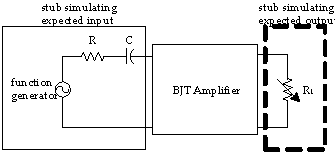
\includegraphics[width=3.8in,height=1.76in]{./image7}
\caption{The use of stubs for testing a transistor amplifier
circuit. The function generator, resistor (R), and capacitor (C) model
the expected behavior of the input source in the final system
implementation. The variable resistance (R\textsubscript{L}) models the
load that would be attached to the output.}
\label{figure:usingStubs}
\end{figure}


\subsection{Test Case Properties}
\label{subsection:test-case-properties}

As we go through the different levels of testing we will need to build
effective test cases. Effective test cases share some common attributes
regardless of their level. Dianne Runnels {[}Run99{]} defined the
following properties for effective test cases:

\begin{itemize}
\item
  \emph{Accurate}. The test should check what it is supposed to and
  exercise an area of intent.
\item
  \emph{Economical}. The test should be performed in a minimal number of
  steps.
\item
  \emph{Limited in complexity}. Tests should consist of a moderate
  number (10-15) of steps.
\item
  \emph{Repeatable}. The test should be able to be performed and
  repeated by another person.
\item
  \emph{Appropriate}. The complexity of the test should be such that it
  is able to be performed by other individuals who are assigned the
  testing task.
\item
  \emph{Traceable}. The test should verify a specific requirement. The
  corresponding requirements for the different types of test are derived
  from the associated development stages in the test vee in Figure 7.1.
\item
  \emph{Self cleaning}. The system should return to the pre-test state
  after the test is complete.
\end{itemize}

\section{Constructing Tests}
\label{section:constructing-tests}

This section presents the four different types of test shown in Figure
7.1 - debugging, unit testing, integration testing, and acceptance
testing. This is presented in reverse order from the order in which test
should be created, as the reader is probably most familiar with basic
test techniques such as debugging. Thus the presentation is from the
most familiar to the more abstract. The next section presents a case
study that proceeds in the opposite direction from acceptance testing to
unit testing.

\subsection{Debugging}
\label{subsection:debugging}

At some point in the design process, the implementation level must be
reached, where tasks such as constructing circuits, wiring integrated
circuits, and writing code are carried out. Applying the functional
decomposition paradigm introduced in Chapter 5 should provide a clear
idea of the inputs, outputs, and behavior of the modules that are being
built. Inevitably, there will come a point during the construction of a
component when it will not function as expected. This is commonly
referred to as a \emph{\textbf{bug}}. It requires the application of
debugging skills to determine the root cause of the problem and correct
it. You have undoubtedly run across a variety of bugs in your day, and
it is a good guess that your bugs fell into one of two camps---Bohrbugs
and Heisenbugs.

\emph{\textbf{Bohrbugs}} are named after the Bohr model of the atom that
assumes that electrons have a distinct position in space. Bohrbugs are
reliable bugs, in which the error is always in the same place. This is
analogous to the electrons having a definite position. Given a
particular input, a Bohrbug will always manifest itself in the same way
and in the same place. Finding a Bohrbug is a matter of laying the
correct trap. A good trap is simple to set-up, quickly causes an error,
and reveals the source of the error. This is a tall order, but one which
experience hones.

\emph{\textbf{Heisenbugs}} are named after the Heisenberg Uncertainty
Principle, in which the position of an electron is uncertain.
Analogously, Heisenbugs may not always be reproducible with the same
input. They seemingly move around within a system and are consequently
difficult to locate. Finding a Heisenbug requires you to think outside
the box because they usually result from unanticipated mechanisms. An
example of a Heisenbug is a computer program with a pointer error that
occasionally overwrites the system stack. This can cause return values
from a subroutine to be incorrect. In such a case, the subroutine would
appear to have a problem, since it is returning the wrong value.
However, testing the subroutine by itself would confirm that the
subroutine works properly. Another good example is a circuit that works
fine on some days, but doesn\textquotesingle t work on others (typically
when a professor is nearby). Insidious problems such as a floating
ground line often are to blame.

Regardless of the bug type, the debugging process is iterative. You must
run tests and depending on the results, go back and run new tests. With
this in mind, you should enter into the debugging process with a
strategy in mind. This strategy is often similar to programming an
if-then structure---``if the test is negative, then I\textquotesingle ll
pursue this line of attack; otherwise the error could be in another
subsystem.'' In general, the debugging process is much the same as the
scientific method. The steps of the debugging process are:

\begin{itemize}
\item
  Observe. Observe the problem under different operating conditions.
\item
  Hypothesize. Form a hypothesis as to what the potential problem is.
\item
  Experiment. Conduct experiments to confirm or eliminate the
  hypothesized source of the problem.
\item
  Repeat. Repeat until the problem is eliminated.
\end{itemize}

When hypothesizing, make sure to check the simplest and easiest
potential problems first. There are two good reasons for this---they are
easy to perform and more tests can be performed in a given period of
time. In addition, designs should be verified from the lowest levels of
abstraction to the highest. For example, voltages should be verified as
correct before moving to higher levels of functionality. The reason for
this heuristic is obvious---the higher level of functionality cannot
operate correctly unless all the lower levels are working.

\subsection{Unit Testing}
\label{subsection:unit-testing}

A \emph{\textbf{unit test}} is a complete test of a module's
functionality. In order to be a complete check, a unit test consists of
a set of test cases each of which establishes that the module performs a
single unit of functionality to some specification. Test cases should be
written with the express intent of uncovering undiscovered defects. For
example, consider a hardware module which converts an input Celsius
temperature into an output Fahrenheit temperature. Let the operation of
the module be represented by the following pseudo-code.

\begin{verbatim}
if (16 < input < 32)
        output = ROM[input -16];
else
        output = (2 * input) + 32;
\end{verbatim}

When the input temperature is between 16 and 32, the output is
determined by a lookup operation in a ROM, otherwise the input is
converted using an approximation to the familiar Celsius to Fahrenheit
conversion. Each test case for this hardware module should exercise a
single area of intent. Clearly, we need to have at least two test cases,
one for the ``if'' clause and one for the ``else'' clause. In addition,
it would be a good idea to check the boundary conditions separating the
``if'' and ``else'' clauses. Finally, we should consider the extreme
values of the input. For example, if the input were a signed 8-bit
number then we should check -128, and 128. If the input is a signed
value then 0 is also a boundary value that should be checked.

This example illustrates the concept of a \emph{\textbf{processing
path}} -- a sequence of consecutive instructions or states encountered
from the beginning to the end of a computation pr process. The
temperature conversion example has two processing paths, one where the
``if'' statement is taken and one when the ``else'' statement is taken.
Each such processing path through the system represents a potential test
case. The extent to which the test cases cover all possible processing
paths is called the \emph{\textbf{test coverage}.} It is desirable to
design test sets that have the highest coverage as possible in the
fewest number of test cases. The ultimate in coverage is achieved by
\textbf{\emph{path-complete coverage}} where every possible path has a
test. However this level of coverage may not be possible because the
number of processing paths goes up exponentially with the number of
nested branches. In cases where there are more paths than it is possible
to check, you must be satisfied with partial path coverage. In such
cases, those paths that which are though to most likely reveal an error
should be tested.

Clearly documenting unit tests has added importance because the test
cases are generally written by one person or group and performed by a
separate group. In order to organize the test cases they can be
organized as matrices, step-by-step tests or automated scripts.

\subsection*{Matrix Tests}
\label{subsection:matrix-tests}

A \emph{\textbf{matrix test}} is a test that is best suited to cases
where the inputs submitted are structurally the same and differ only in
their values. The test procedure is then ``factored out'' leaving a list
of inputs and their expected outputs. Since the tests are written by one
group and performed by another the test writer must leave space in the
test document for the tester to make comments and observations regarding
the system behavior.

Lets consider a test for the analog-to-digital converter (ADC) that was
used in the temperature measuring system in Chapter 5 (Section 5.7,
Figure 5.11). Assume that the ADC's clock frequency is 10 kHz and the
input ranges from 0 to 5 volts. The unit test will consist of submitting
different inputs to the ADC and verifying the outputs. Since each test
only varies the input, with no change in the testing procedure, the test
matrix in Table 7.1 was created.

This test case exercises each bit of the ADC's output independent of the
other output bits. Other test cases should examine extreme inputs as
well as illegal inputs. Care should be taken that illegal inputs do not
stress the ADC beyond the manufactures recommendations; otherwise the
tests might accidentally damage the ADC.

\textbf{\hfill\break
Table 7.1} A matrix test for an analog-to-digital converter.

\begin{table}
\caption{}
\label{table:<context>}
\begin{tabular}{|m{1cm}|m{2cm}|m{2cm}|m{2cm}|m{1cm}|m{1cm}|m{1cm}|m{2cm}|}
\hline

\multicolumn{8}{l} {\textbf{Test Writer:} Sue L. Engineer}\\ \hline

\multicolumn{2}{l} {\textbf{Test Case Name:}} &
\multicolumn{2}{l} {ADC unit test} &
\multicolumn{3}{l}{\textbf{Test ID \#:}} & ADC-UT-01 \\ \hline

\multicolumn{2}{l} {\textbf{Description:}}&
\multicolumn{2}{l} {Verify that each bit of the output can be set independently of the other outputs.} &
\multicolumn{3}{l}{\textbf{Type:}} &  white box or black box \\ \hline

\multicolumn{8}{l} {\textbf{Tester Information}} \\ \hline

\multicolumn{2}{l} {\textbf{Name of Tester:}} &
\multicolumn{2}{l} { } &
\multicolumn{3}{l}{\textbf{Date:}} &  \\ \hline

\multicolumn{2}{l} {\textbf{Hardware Ver:}} &
\multicolumn{2}{l} { 1.0} &
\multicolumn{3}{l}{\textbf{Time:}} &  \\ \hline

\multicolumn{2}{l} {\textbf{Setup:}}&
\multicolumn{6}{l} {Isolate the ADC from the system by removing configuration jumpers.
Connect the clk input to a 10 KHz clock source and the Din input to a
high precision voltage course. Connect the output from the ADC to a
logic analyzer.}   \\ \hline


\textbf{Test} & $V_T$ & 
\multicolumn{2}{l}{\textbf{Expected output}} & 
\textbf{Pass} &
\textbf{Fail} & 
\textbf{Comments} \\  \hline

1 & 0.000 V & 0 & 0x000 & & & & \\ \hline
2 & 0.004887 V & 1 & 0x001 & & & & \\ \hline
3 & 0.00977 V & 2 & 0x002 & & & & \\ \hline
4 & 0.01955 V & 4 & 0x004 & & & & \\ \hline
\ldots{} & \ldots{} & \ldots{} & \ldots{} & & & & \\ \hline
10 & 2.502 V & 512 & 0x200 & & & & \\ \hline

\multicolumn{3}{l}{\textbf{Overall test result:}} &   &  &  & \\ \hline
\end{tabular}
\end{table}

\subsection*{Step-by-Step Tests}
\label{subsection:step-by-step-tests}

A \emph{\textbf{step-by-step test}} case is a prescription for
generating the test and checking the results. These descriptions are
most effective when the test consists of a complex sequence of steps.
The test template for a step-by-step test has the all information
contained in the matrix test template the difference being the addition
of a column in the test section describing what action the tester should
perform at each step in the test process.

As an example, recall the state diagram for the vending machine in
Chapter 6 (Figure 6.2) that accepts nickels and dimes and dispenses
candy when a total of \$0.25 (or more) is submitted. The state machine
has different processing paths, depending upon the combination and order
of coins deposited. Test cases can be written for each of the processing
paths through the system, and an example is shown in 
Table~\ref{table:stepByStepTest} for one
particular processing path.


\begin{table}
\caption{A step-by-step test for a vending machine.}
\label{table:stepByStepTest}
\begin{tabular}{|m{1cm}|m{2cm}|m{2cm}|m{1cm}|m{1cm}|m{1cm}|m{2cm}|m{2cm}|}
\hline

\multicolumn{8}{l} {\textbf{Test Writer:} Sue L. Engineer}\\ \hline

\multicolumn{2}{l} {\textbf{Test Case Name:}} &
\multicolumn{4}{l} {Finite State Machine Path Test \#1} &
\multicolumn{1}{l}{\textbf{Test ID \#:}} & FSM-Path-01 \\ \hline

\multicolumn{2}{l} {\textbf{Description:}}&
\multicolumn{4}{l} {Simulate insertion of money with a mix of nickels and dimes. Verifies
FSM outputs candy in response to a total deposit of \$0.30.} &
\multicolumn{1}{l}{\textbf{Type:}} &  white box or black box \\ \hline

\multicolumn{8}{l} {\textbf{Tester Information}} \\ \hline

\multicolumn{2}{l} {\textbf{Name of Tester:}} &
\multicolumn{4}{l} { } &
\multicolumn{1}{l}{\textbf{Date:}} &  \\ \hline

\multicolumn{2}{l} {\textbf{Hardware Ver:}} &
\multicolumn{4}{l} { 1.0} &
\multicolumn{1}{l}{\textbf{Time:}} &  \\ \hline

\multicolumn{2}{l} {\textbf{Setup:}}&
\multicolumn{6}{l} {Make sure that the system was reset sometime prior and is in state \$0.00}   \\ \hline

\textbf{Step} & \textbf{Action} &  \textbf{Expected Result} & 
\textbf{Pass} & \textbf{Fail} &  \multicolumn{2}{l}{\textbf{Comments}} \\  \hline
1 & Strobe Nickel & State should go to \$0.05 & & & & \multicolumn{2}{l}{} \\ \hline
2 & Strobe Dime & State should go to \$0.15 & & & & \multicolumn{2}{l}{}\\ \hline
3 & Wait & State should remain \$0.15 & & & & \multicolumn{2}{l}{}\\ \hline
4 & Strobe Nickel & State should go to \$0.20 & & & & \multicolumn{2}{l}{}\\ \hline
5 & Strobe Dime & State should go to \$0.25 & & & & \multicolumn{2}{l}{}\\ \hline
6 & Nothing & State should go to \$0.00 & & & & \multicolumn{2}{l}{}\\ \hline
\multicolumn{3}{l}{\textbf{Overall test result:}} &   &  &  & \multicolumn{2}{l}{}\\ \hline
\end{tabular}
\end{table}


\subsection*{Automated Test Scripts}
\label{subsection:automated-test-scripts}

An \emph{\textbf{automated test}} \emph{\textbf{script}} is a sequence
of commands provided to the UUT without user intervention. The outputs
are usually automatically compared against the expected outputs to
determine if the module contains an error. Automated scripts are
executed from a device referred to by many different names like test
harness, test fixture, and test bench.

While automated scripts carry a lot of up front cost in terms of the
time required putting them together they pay dividends when performing
\emph{\textbf{regression testing}}. Regression testing is the process of
retesting a module following a modification in any related part of the
system to ensure that no errors were inadvertently introduced. Reducing
the time spent on regression testing will has a positive effect on the
overall development time. Hence, the benefit of automated scripts is
realized later in the testing cycle. In addition, design decision can
have an effect on the amount of time spent on regression testing. It
stands to reason that systems with highly coupled modules require more
extensive and consequently more time consuming regression testing.

The template for the matrix tests could be used to describe what an
automated test script does. However, the specifics of how the automated
scripts perform these actions are implementation specific. For example,
in hardware description languages the stimulus and responses of the UUT
are processed by a test bench. The test bench is itself a piece of
hardware coded in the same hardware language used to describe the UUT.

\subsection{Integration Testing}
\label{subsection:integration-testing}

After the individual subsystems have undergone their unit tests, they
are then integrated into large subcomponents leading eventually to the
construction of the entire system. Hence \emph{\textbf{integration
testing}} checks that the major modules of the overall system operate
correctly together. The test cases for integration testing must be
traceable to the high-level design, and the test cases are written based
on characteristics of the design architecture. Test cases for
integration can be derived from the following questions:

\begin{itemize}
\item
  Have all the execution paths through the system been exercised?
\item
  Have all the modules been exercised at least once?
\item
  Have all the interface signals been tested?
\item
  Have all interface modes been exercised?
\item
  Does the system meet timing requirements?
\end{itemize}

The integration tests themselves can be documented using either the
matrix or step-by-step template outlined for unit tests.

\subsection{Acceptance Testing}
\label{subsection:acceptance-testing}

An \emph{\textbf{acceptance test}} is a formal document stipulating the
conditions under which the customer will accept the system. It generally
consists of a suite of test cases that exercise the systems according to
the user's environment. The test cases are constructed to ensure that
the engineering requirements are met. The four attributes of a good
requirement (abstract, unambiguous, traceable, and verifiable) are
important in building a good acceptance test. An unambiguous requirement
will result in a test which everyone can agree on. A verifiable
requirement sets an objective pass/fail criterion on the acceptance
test. Tests based on a traceable requirement imply they are directly
assessing the needs of the project. However, an acceptance test goes far
beyond an enumeration of the test cases. It typically includes the
following sections:

\begin{itemize}
\item
  Testing Approach. The types, level and methods employed to test the
  system.
\item
  Test Schedule. Start and end dates for the individual tests.
\item
  Problem Reporting. How the test results will be recorded.
\item
  Resource Requirements. The hardware, software, and people requirements
  needed to perform the tests.
\item
  Test Environment. The setup required to run the tests.
\item
  Test Equipment. Any special equipment or configurations required to
  run the test.
\item
  Post-Delivery Tests. Tests performed on the deployed system.
\item
  Test Identification. Enumeration of test cases and their unique
  identifiers.
\item
  Corrective Action. What repairs must be made to the system in order to
  accept it.
\end{itemize}

It is not necessary for every test case to be passed in order for the
system to be accepted. The acceptance test should stipulate the degree
of importance surrounding each test. While it's easy to imagine writing
the test cases for an acceptance test, the process can become a
chicken-and-egg problem. That is you are trying to stipulate the test
procedures and results for a system which has yet to be implemented of
the system. This can often lead to revisions of the acceptance test plan
later in the design cycle.

\section{Case Study: Security Robot Design}
\label{section:case-study-security-robot-design}

In order to demonstrate the concepts involved in testing lets consider
the design of a security system which monitors an office complex looking
for intruders. The design team has decided to address the need by
designing a mobile robot which autonomously navigates its way through
the office space. The team, along with the customer, developed a number
of requirements and from this we will focus on two that address a
fundamental navigational problem.

\begin{itemize}
\item
  \emph{The robot's center must stay within 12 to 18 centimeters of the
  wall over 90\% of the course, while traveling parallel to a wall over
  a 3 meter course.}
\item
  \emph{The robot's heading should never deviate no more than 10 degrees
  from the wall's axis, while traveling parallel to a straight wall over
  a 3 meter course.}
\end{itemize}

This case study explores test cases for the acceptance, integration and
unit testing related to these two requirements. The development of the
test cases follows the proper order of test case development illustrated
in Figure 7.1. That means acceptance tests are developing in conjunction
with the requirements, integration tests are constructed during the
system design, and unit tests during the system build.

\subsection*{Acceptance Testing}
\label{subsection:acceptance-testing-1}


We start by constructing an acceptance test case to verify that the
robot can achieve the stated requirements. A number of tests would need
to be built and we create a test only for the first engineering
requirement. A test could be performed by having someone observe the
robot moving along a wall and mark (on the floor) whenever the robot
strayed out of bounds. Such a test would not easily be repeatable
because different people might judge what is meant by ``out of bounds''
differently. The accuracy of such a test is questionable because
determining when and if a speeding robot crossed the boundary is
difficult. Finally, there would be no permanent record of the test
results making it difficult for the customer to actually verify the test
was passed. A way to address these problems is to have the robot monitor
its own distance from the wall. This is done in this case by a program
written to monitor the position of the robot over time and store these
values. From the specifications for a step-by-step acceptance in 
Table~\ref{table:stepByStepAcceptanceTestRobot}
it is clear what the test program must configure the robot to log
the distance data while traversing the wall. After this data is
downloaded from the robot it can be analyzed in a spreadsheet program to
determine the needed metrics and archived for future reference.

\begin{table}
\caption{A step-by-step acceptance test case for the autonomous robot.}
\label{table:stepByStepAcceptanceTestRobot}
\begin{tabular}{|m{1cm}|m{2cm}|m{2cm}|m{1cm}|m{1cm}|m{1cm}|m{2cm}|m{2cm}}
\hline

\multicolumn{8}{l} {\textbf{Test Writer:} Sue L. Engineer}\\ \hline

\multicolumn{2}{l} {\textbf{Test Case Name:}} &
\multicolumn{4}{l} {Robot Acceptance Test \#1} &
\multicolumn{1}{l}{\textbf{Test ID \#:}} & Robot-AT-01 \\ \hline

\multicolumn{2}{l} {\textbf{Description:}}&
\multicolumn{4}{l} {The robot's center must stay
within 12 to 18 centimeters of the wall over 90\% of the course, while
traveling parallel to a wall over a 3 meter course.} &
\multicolumn{1}{l}{\textbf{Type:}} &  white box or black box \\ \hline

\multicolumn{8}{l} {\textbf{Tester Information}} \\ \hline

\multicolumn{2}{l} {\textbf{Name of Tester:}} &
\multicolumn{4}{l} { } &
\multicolumn{1}{l}{\textbf{Date:}} &  \\ \hline

\multicolumn{2}{l} {\textbf{Hardware Ver:}} &
\multicolumn{4}{l} {Robot 1.0} &
\multicolumn{1}{l}{\textbf{Time:}} &  \\ \hline

\multicolumn{2}{l} {\textbf{Setup:}}&
\multicolumn{6}{l} {Completed robot should be fully charged and placed on 3 meter test track.}   \\ \hline

\textbf{Step} & \textbf{Action} &  \textbf{Expected Result} & 
\textbf{Pass} & \textbf{Fail} & \multicolumn{2}{l}{ \textbf{Comments}} \\  \hline
1 & Write a program to monitor the robots position from the wall. &
Program should be statically tested to verify accuracy. Should sample
wall at a sufficient rate depending on speed. & & & &\multicolumn{2}{l}{}\\ \hline
2 & Put robot on test track, run test, and download data. & The robot
should travel down the entire length of the test track and then stop. &
& & &\multicolumn{2}{l}{}\\ \hline
3 & Plot test data in a spreadsheet program. & Plot of position vs. time
should be within 12 -- 18 cm 90\% of the time. & & & &\\ \hline
\multicolumn{3}{l}{\textbf{Overall test result:}} &   &  &  & \multicolumn{2}{l}{}\\ \hline
\end{tabular}
\end{table}

\subsection*{Integration Testing}
\label{subsection:integration-testing-1}

The team, in consultation with the customer, has gone through the
requirements and created a complete set of acceptance tests in addition
to the test in Table 7.3. They next turn to developing a high level
design architecture that can meet the requirements. The design they
create is shown in 
Figure~\ref{figure:level1mobileRobot}, the Level 1 architecture of the
autonomous robot.


\begin{figure}
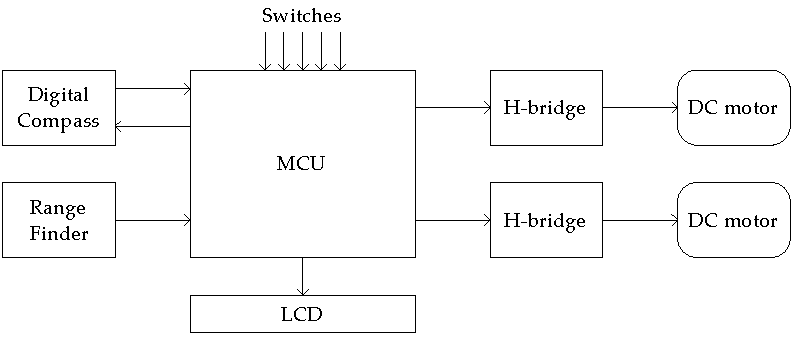
\includegraphics[width=4.9in,height=2.1in]{./image8}
\caption{Level 1 design architecture for the mobile robot.}
\label{figure:level1mobileRobot}
\end{figure}

The heart of the design is a microcontroller (MCU) which reads the
sensor values, makes decisions, and controls the speed of the two drive
motors. The robot moves and turns by adjusting the relative speed of
each motor using a pulse-width modulated (PWM) signal from the MCU. The
duty cycle of the PWM is directly proportional to the speed of the
motor. The H-bridges then amplify the MCU output to power to the motors.
The MCU also outputs a set of signals to send text to an LCD. The signal
to the digital compass is bidirectional because the MCU must configure
the operating mode of the compass before using it. The MCU receives an
analog input from the range finder, where the voltage level of the
signal is proportional to the distance to the obstacle. Finally, a set
of switches are included that allow for manual input and testing of the
robot.

Clearly, the interaction of the MCU with each of the compass,
rangefinder, LCD, switches, and H-bridges should be examined. However,
this will be left to the unit test because the MCU makes a great test
harness which can be used to provide stimulus to and read outputs from
these I/O. In addition, many of the routines from these tests can be
reused later in the development process.

There are many interactions between subsystems that could be tested
during integration testing. A careful examination of the system must be
done to determine which combinations of subsystems are most likely to
create problems. Experience and component selection play a large part in
molding expectations. For example, the magnetic field created by the
windings in the DC motor can affect the reading generated by the
compass. This interaction could potentially affect the headings read by
the MCU and cause the robot to go off course by more than the allowable
10 degrees. Thus a step-by-step integration test is created in 
Table~\ref{table:stepByStepIntegrationTestRobot}
to test the operation of the motors with the magnetic compass.


\begin{table}
\caption{A step-by-step integration test case for the compass and motors.}
\label{table:stepByStepIntegrationTestRobot}
\begin{tabular}{|m{1cm}|m{2cm}|m{2cm}|m{1cm}|m{1cm}|m{1cm}|m{2cm}|m{2cm}|}
\hline

\multicolumn{8}{l} {\textbf{Test Writer:} Sue L. Engineer}\\ \hline

\multicolumn{2}{l} {\textbf{Test Case Name:}} &
\multicolumn{4}{l} {Robot Integration Test \#1} &
\multicolumn{1}{l}{\textbf{Test ID \#:}} & Robot-IT-01 \\ \hline

\multicolumn{2}{l} {\textbf{Description:}}&
\multicolumn{4}{l} {Checks interaction of DC motors on the magnetic compass.} &
\multicolumn{1}{l}{\textbf{Type:}} &  white box or black box \\ \hline

\multicolumn{8}{l} {\textbf{Tester Information}} \\ \hline

\multicolumn{2}{l} {\textbf{Name of Tester:}} &
\multicolumn{4}{l} { } &
\multicolumn{1}{l}{\textbf{Date:}} &  \\ \hline

\multicolumn{2}{l} {\textbf{Hardware Ver:}} &
\multicolumn{4}{l} {Robot 1.0} &
\multicolumn{1}{l}{\textbf{Time:}} &  \\ \hline

\multicolumn{2}{l} {\textbf{Setup:}}&
\multicolumn{6}{l} {A wooden turn-table should be placed on top of the cardinal direction
map. This map should be aligned with a magnetic compass. There should be
no metal present while the alignment is being performed. Next, the
partially assembled robot should be placed on the turn-table. The MCU
should be connected to a terminal to observe and record data.}   \\ \hline

\textbf{Step} & \textbf{Action} &  \textbf{Expected Result} & 
\textbf{Pass} & \textbf{Fail} & \multicolumn{2}{l}{ \textbf{Comments}} \\  \hline

1 & Write program to spool compass readings while simultaneously driving
motors. & Program should be statically tested to verify accuracy. Should
sample compass at a sufficient rate depending on speed. & & & & \multicolumn{2}{l}{} \\ \hline
2 & Run acceptance test & Test program should prompt user to turn the
robot to an orientation and then spin the motors will then spin up and
down. & & & & \multicolumn{2}{l}{}\\ \hline
3 & Plot spooled data in spreadsheet program. & Plots should be analyzed
to see if compass deviated any more than 10 degrees from set point. & &
& &\multicolumn{2}{l}{}\\ \hline

\multicolumn{3}{l}{\textbf{Overall test result:}} &   &  &  & \multicolumn{2}{l}{}\\ \hline
\end{tabular}
\end{table}

It is clear from this test case that a testing program needs to be
written in order to prompt the user to align the robot, capture compass
readings, and then to spool them back to the user. The requirement that
the compass readings deviate no more than 10 degrees is based on the
engineering requirement that the robot deviate no more than 10 degrees
from the walls axis while navigating down the hallway.

\subsection*{Unit Testing}
\label{subsection:unit-testing-1}


Once the Level 1 architecture is developed and the test cases written to
ensure that the architecture is capable of meeting the design
requirements, the design team moves on to selecting components to use in
the design. The design team must select the units so that the resulting
system can meet the engineering requirements. Each of the individual
components Figure~\ref{figure:level1mobileRobot}
needs to be considered as a candidate for unit
testing. In general each functional unit might have several test cases
comprising its unit test. A unit test for the digital compass component
will illustrate this. Prior to presenting the test case, the functional
design requirements for the unit are given in 
Table~\ref{table:functionalDigitalCompass}.


\begin{table}
\caption{The functional requirements for the digital compass.}
\label{table:functionalDigitalCompass}
\begin{tabular}{|l|m{10cm}|}
\hline
\emph{Module} & Digital Compass -- Geosensor version 2.3 \\ \hline
\emph{Inputs} & 
\begin{itemize}
\item
  Earth's magnetic field: An orientated field of magnetic force
  beginning and ending at the earth's magnetic poles.
\item
  SClk -- Clock signal to clock data through the module. Maximum
  Frequency is 10Mhz.
\item
  SDIn -- Serial data input to send data into the compass module. Date
  is valid on positive SClk edges.
\end{itemize}\\ \hline
\emph{Outputs} & 
\begin{itemize}
\item
  SDOut -- Serial data output from the compass module. Data is valid on
  negative clock edges.
\end{itemize}\\ \hline
\emph{Functionality} & Senses the earth's magnetic field and determines
the orientation of the compass with respect to the field. This
orientation is stored in an internal register and can be retrieved
through the SPI interface. \\ \hline
\emph{Test} & Comp-UT-01 \\  \hline
\end{tabular}
\end{table}

In order to be useful in the overall design the compass module must be
able to accurately report the robot's heading. The requirements place an
upper bound of 10 degrees on the error in the heading of the robot.
Thus, the matrix test case is Table~\ref{table:matrixTestDigitalCompass}
is constructed to configure the
compass and then reads heading data from it. This unit test looks for
heading errors greater than 10 degrees.

\textbf{Table 7.6} 
\begin{table}
\caption{Matrix unit test for the digital compass.}
\label{table:matrixTestDigitalCompass}
\begin{tabular}{|m{1cm}|m{2cm}|m{2cm}|m{1cm}|m{1cm}|m{1cm}|m{2cm}|m{2cm}|}
\hline

\multicolumn{8}{l} {\textbf{Test Writer:} Sue L. Engineer}\\ \hline

\multicolumn{2}{l} {\textbf{Test Case Name:}} &
\multicolumn{4}{l} {Compass Unit Test \#1} &
\multicolumn{1}{l}{\textbf{Test ID \#:}} & Comp-UT-01 \\ \hline

\multicolumn{2}{l} {\textbf{Description:}}&
\multicolumn{4}{l} {Checks that the compass returns correct angular measurements to the MCU.
Test program is in ./test/compass\_unit\_test\_1.c} &
\multicolumn{1}{l}{\textbf{Type:}} &  white box or black box \\ \hline

\multicolumn{8}{l} {\textbf{Tester Information}} \\ \hline

\multicolumn{2}{l} {\textbf{Name of Tester:}} &
\multicolumn{4}{l} { } &
\multicolumn{1}{l}{\textbf{Date:}} &  \\ \hline

\multicolumn{2}{l} {\textbf{Hardware Ver:}} &
\multicolumn{4}{l} {Compass Module - Geosensor version 2.3} &
\multicolumn{1}{l}{\textbf{Time:}} &  \\ \hline

\multicolumn{2}{l} {\textbf{Setup:}}&
\multicolumn{6}{l} {Compass module should be wired to the MCU through the SPI interface
pins. The MCU should be connected to an RS232 terminal through its SCI
interface. The terminal should be configured to run at 9600 baud.
Cardinal directions map should be aligned using the magnetic
compass.}   \\ \hline

\textbf{Step} & \textbf{Action} &  \textbf{Expected Result} & 
\textbf{Pass} & \textbf{Fail} & \multicolumn{2}{l}{ \textbf{Comments} }\\  \hline


1 & Compile compass.c in /test directory & IDE should generate no
warnings or errors. & & & & \multicolumn{2}{l}{}\\ \hline

2 & Download & MCU should report ``download successful'' & & & & \multicolumn{2}{l}{}\\ \hline

3 & Execute & MCU should display compass splash screen on terminal
interface. & & & & \multicolumn{2}{l}{}\\ \hline

4 & Orientate compass to 0 degrees. & Terminal interface should display
0 degrees +/- 10 degrees. & & & & \multicolumn{2}{l}{}\\ \hline

5 & Orientate compass to 30 degrees. & Terminal interface should display
30 degrees +/- 10 degrees. & & & & \multicolumn{2}{l}{}\\ \hline

6 & Orientate compass to 45 degrees. & Terminal interface should display
45 degrees +/- 10 degrees. & & & & \multicolumn{2}{l}{}\\ \hline

\ldots{} & \ldots{} & \ldots{} & & & &  \multicolumn{2}{l}{}\\ \hline

12 & Orientate compass to 315degrees. & Terminal interface should
display 315 degrees +/- 10 degrees. & & & & \multicolumn{2}{l}{}\\ \hline
\multicolumn{3}{l}{\textbf{Overall test result:}} &   &  &  &  \multicolumn{2}{l}{}\\ \hline
\end{tabular}
\end{table}

\section{Guidance}
\label{section:guidance}

Tests have a lifetime beyond the obvious need to check proper operation
of the subsystems, their integration, and the overall performance of the
system. Test cases describe how the system operates in plain English.
Test cases can be used to develop diagnostics, assist in writing
technical documentation, and aid marketing and sales staff in
understanding system performance. Testing is a value-added process in
design. Beyond attempting to remove bugs from the system, Burke and
Coyner {[}Bur03{]} suggest the following are good reasons to perform
testing:

\begin{itemize}
\item
  \emph{Testing reduces the number of bugs in existing and new
  features}. Testing does not eliminate all the bugs, but rather reduces
  the probability of a bug making it to production.
\item
  \emph{Tests are good documentation}. Tests provide insight to others
  on the operation of the unit under test and how to interface to it.
\item
  \emph{Tests reduce the costs of change}. A change to a complex design
  with no tests can produce bugs that are difficult to track down. A
  good set of regression tests can help localize the effect of bugs
  introduced by changes.
\item
  \emph{Tests improve design}. In order to create a testable design, you
  need to create highly cohesive, loosely coupled units.
\item
  \emph{Tests allow you to refactor}. Subcomponents of a testable design
  can be changed and optimized with less chance of introducing new
  errors. This is because tests exist that can verify the redesigned
  (refactored) module functions correctly.
\item
  \emph{Tests constrain features}. When a test is written before
  building the associated module, the exact requirements are defined.
  Hence, when a unit passes its test, there is confidence that the
  requirements have been met.
\item
  \emph{Tests defend against other designers}. Often a design needs to
  have circuitry to deal with special cases. Tests that check these
  special cases can make sure that future modification do not remove
  them.
\item
  \emph{Testing is fun}. Writing tests requires creative solutions to
  complex design problems.
\item
  \emph{Testing forces you to slow down and think}. When writing a test
  before incorporating a feature into a design, you are forced to see
  how the new feature fits into the existing design framework.
\item
  \emph{Testing makes development faster}. On a component level, testing
  slows development. However, as the design becomes larger and more
  complex, modules can be more easily integrated into the design without
  causing malfunctions in existing components.
\item
  \emph{Tests reduce fear}. Would you rather improve a unit with a test
  suite or one without?
\end{itemize}

\section{Summary and Further Reading}
\label{section:summary-and-further-reading}

Testing is an important part of the design process that helps to ensure
systems will operate properly. This chapter examined basic principles of
testing including black box testing, white box testing, controllability,
and observability. They address the manner in which tests can be
conducted, controlled, and states of the system observed. The use of
stubs, which are employed to simulate system inputs and outputs were
examined, as well as the properties of test cases. The different phases
of testing from unit tests through integration tests to acceptance tests
were examined. Testing proceeds from the most detailed level of the
system to the most general, and the tests performed in each phase are
traceable to their corresponding phases in the design development
process.

The field of testing has been well developed by the software engineering
community. \ul{Software Engineering: An Engineering Approach}
{[}Pet00{]} provides a good overview of testing principles such as black
box and white box testing. It also includes a number of test strategies
beyond those considered here. The \ul{Glossary of Vulnerability Testing
Terminology} from the University of Oulu's Electrical and Information
Engineering department {[}Oul04{]} provides an extensive list of terms
related to testing in the software domain. Gray's 1985 article \emph{Why
Do Computers Stop and What Can Be Done About It?} {[}Gra85{]} coined the
terms Heisenbug and Bohrbug. This article introduces many interesting
facts about how supercomputers fail. It provides a rare chance to look
at the inner world of a supercomputer company. Many of the topics in the
unit test section were influenced by Dianne L. Runnel's article
\emph{How to Write Better Test Cases} {[}Run99{]}. In this article, she
defines precisely what is meant by unit test, and gives a clear picture
of how to construct a unit test. This article along with many other
scholarly articles on testing can be found at www.stickyminds.com. An
exceptional set of documents and templates are available from the
Systems Engineering Processing Group of the United States Air Force.
While intended for software development, the checklists for unit and
integration testing contain many insightful points. They are accessible
at

https://ossg.gunter.af.mil/applications/sep/menus/Main.aspx. The list of
acceptance test items was due in part to the information fond at:
http://www.tbs-sct.gc.ca/emf-cag/acceptance/outline/atpo-vper\_e.asp
